\section{How Accurately Does Geometry Predict Blind Reach Distance?} \label{sec:reaching}
To understand how stereo geometry errors in HMDs affect near-field distance perception, and specifically how changes in perceived distance impact reaching behavior, we compared participants' blind reaching errors against the stereo triangulation model described in in Section~\ref{sec:model overview}.

% To understand how stereoscopic geometric errors in HMDs affect distance perception in the near field, we performed a series of blind experiments in an HMD with different rendering and viewing errors. We compared participants' blind reaching errors to the predictions of our simple triangulation model in Section \ref{sec:model overview} to test how well misperceptions of distance in HMDs can explained by errors in stereo geometry alone. 

\subsection{Error Condition Selection} \label{sec:exp1_procedure}
We evaluated three rendering and viewing errors critical to current VR hardware designs (Figure~\ref{fig:error_choices}).

% We measured blind reaching in a real world task to establish a per-subject comparative baseline for in-HMD blind reaching performance and describe the methods to measure each below.
% We ran a series of experiments to examine the conditions outlined in Section~\ref{sec:conditions} and real life blind reaching experiment to establish a comparaitive baseline for our VR reaching tasks.

\paragraph{Direct Passthrough Rendering Error}
Video passthrough headsets can use view reprojection \cite{ElChemalyGAP, xiao2022neuralpassthrough} or computational imaging \cite{kuo23} to correct for the positional offset between the passthrough cameras and the viewer's eyes. Alternatively, "direct passthrough" avoids these computationally expensive methods, and potential image distortions associated with them, by directly streaming perspective-incorrect video. To simulate this effect, we displaced the render cameras by 5.5 cm—a value representative of the thickness of current commercial headsets. We also simulated a -5.5 cm error for completeness (Figure~\ref{fig:error_choices}A).

\paragraph{IPD Viewing Error}
Perceived depth is inherently tied to retinal binocular disparity and a user's IPD. Failure to match the headset's interaxial distance (IAD) to the user's IPD creates a viewing error (not a rendering error because the render cameras and HMD CoP are colocated) and the user will experience incorrect disparity and vergence demand at the fixation point. We picked 12 mm errors based on a worst-case error in real life HMD use (Figure~\ref{fig:error_choices}B).

\paragraph{Eye Relief Viewing Error}
Due to differences in facial geometry, a viewer's actual nominal eye position in the headset may be displaced from this assumed location. We picked 3 cm as a potential eye relief viewing error which represents a value that is as large as could be reasonably expected for a typical HMD optical design (Figure~\ref{fig:error_choices}C).

\subsection{Participants}
Thirty-two participants (mean age: 32.2 years, $\sigma=7.2$; mean IPD: 62.7 mm, $\sigma=2.6$) with normal or corrected-to-normal visual acuity of 20/20 and Randot stereo acuity <= 50 arc seconds participated in the study. All study protocols were IRB approved.

\subsection{Methods}
\paragraph{Real Life Blind Reaching}
To check for inherent reaching biases, participants viewed a physical coin at 30 cm, closed their eyes, and reached for it. During the task, each participant's head was stabilized in a chin rest. A coin was placed on the table at 30 cm away from their forehead by the experimenter and participants were asked to remember its position. They then closed their eyes, after which the coin was removed by the experimenter, and were asked to reach for the coin's location. Participant's eyes remained closed until reach distance was recorded and their arm was back at their side. The participant was not made aware that the coin was placed at the same distance on each trial. This process was repeated three times to assess baseline blind reaching performance in real life.

\paragraph{In Headset Blind Reaching} 
Participants viewed a virtual controller at 30 cm (Figure~\ref{fig:teaser}E), hid the controller via a button press, and reached for the remembered location with a real controller. They had unlimited time to view the virtual controller and pressed a button on the left controller to hide the target when they were ready to start their reach with the right controller. Once they were satisfied with their controller placement, participants pressed another button on the left controller to record the right controller's position, and returned their right hand with the controller to a comfortable resting position. There were seven conditions in total: $\pm$ 55 mm direct passthrough rendering error, $\pm$ 12 mm IPD viewing error, $\pm$ 30 mm eye relief error, and a no error condition. The testing order of conditions was random and participants completed a total of 210 trials (30 trials for each condition) in a single session. Participants were asked to minimize head movement. An outlier analysis was performed for each condition to remove trials that appeared to be inadvertent completions where at least one of three coordinates of the controller was recorded beyond lower or upper fences (1st quartile - 1.5 times the interquartile range (IQR) or 3rd quartile + 1.5 IQR) of the recorded reach positions. On average this led to the removal of 2 trails ($\sigma$ = 1.7) per condition (30 trials).


\paragraph{Data Transforms}
Two transforms were applied to the reaching data. First we apply bias correction to account for each participant's baseline blind-reaching bias from the real-life reach (Figure~\ref{fig:bias_plot}, right marker). These transformed values are shown in Figure~\ref{fig:reaching_HMD_coordinates} (right marker of each panel). For the second transform, we converted distances from HMD coordinates to egocentric coordinates (Section \ref{sec:model overview}) since perceived distance by definition is in an egocentric coordinate frame. The transformed egocentric distance values are shown in Figure~\ref{fig:reaching_egocentric_coordinates}. This second transform only affects values in the eye relief error condition as HMD coordinate frame and egocentric coordinate frame are offset by 3 cm (Figure \ref{fig:error_choices}C). 

\subsection{Statistics}
Linear mixed effects models (LMEM) were used to estimate the influence of rendering and viewing errors on the magnitudes of reaching errors. In all cases, we specified a maximal model by default (i.e., including random intercepts and slopes for all relevant factors) following \cite{Barr2013RandomES,Harrison2018ABI, MixedEffectsLME4, maxwell2017StatsBooks}. For the reaching data, the maximal model was

\begin{equation}
\begin{split}
    \text{reachBias} \sim \text{error}
    + \space (\text{error} \mid \text{ID})
\end{split}
\end{equation}

where error was the magnitude in centimeters of the rendering or viewing error — for example, for direct passthrough: -5.5, 0, or 5.5 cm; reachBias was the bias of the average reach endpoint in egocentric coordinates, after also subtracting off any biases observed in the 0 cm / no-error condition. ID was simply each participant ID. 

\begin{figure}
	\centering
	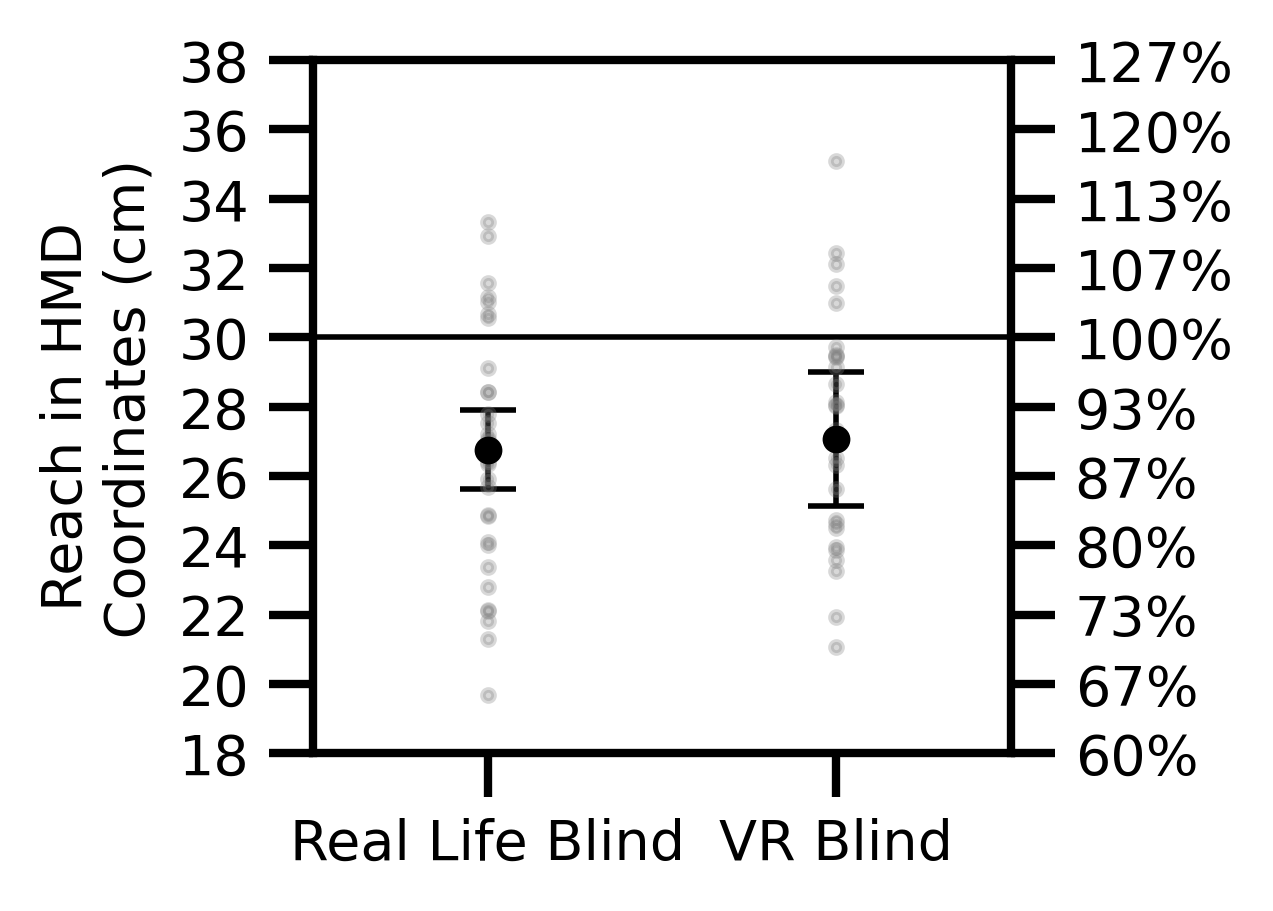
\includegraphics[width=0.65\linewidth]{figures/reaching/real_life_VR_reaching_comparison.png}
	\caption{Blind reaching with correct stereo geometry (no viewing or rendering errors). Black points show the average reach distance and 95\% confidence intervals across all participants (n=32) for a target positioned 30 cm away in HMD coordinate system. Grey points show individual participant data. On average, participants under-reach in both real-life and VR blind reaching conditions by approximately 10\%. 
	}
	\label{fig:bias_plot}
\end{figure}


\begin{figure}[]
    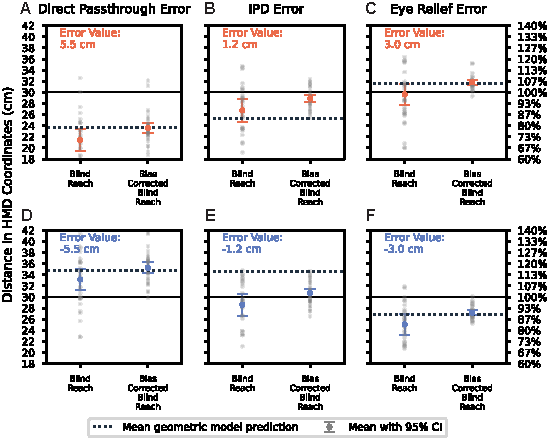
\includegraphics[width=\linewidth]{figures/reaching/reaching_HMD_coordinates.pdf}
    \caption{Reach distance in HMD coordinates for blind reaching and blind reaching corrected for under-reaching bias for \textbf{(A)} direct passthrough error, \textbf{(B)} IPD error, and \textbf{(C)} eye relief error. Positive errors are shown in the top row (red) and negative errors are shown in the bottom row (blue). Black points are means with error bars denoting 95\% confidence interval (n=32). After accounting for participant under-reaching bias, blind reach distances are well-predicted by our model for direct passthrough error and eye relief error.}
    \label{fig:reaching_HMD_coordinates}
\end{figure}

\subsection{Results}
\label{sec:exp1results}
Geometric errors induced statistically significant changes in perceived distance across all conditions. Notably, the magnitude of these shifts aligned closely with geometric predictions for direct passthrough and eye relief errors. In contrast, the observed effect of IPD error, while significant, was substantially smaller than the geometric model predicted.

\paragraph{No Rendering or Viewing Error}
Participants consistently under-reached the $30$~cm target (hypometric reaching) in both VR and real-world baselines (Figure~\ref{fig:bias_plot}). Across 32 participants, endpoints fell short by approximately $3$--$4$~cm ($\sim10\%$). The difference between real-world and VR performance was not statistically significant (paired t-test: $t = 0.71, p = 0.47, df = 31$), suggesting that the under-reaching observed in this study shares a common etiological origin with natural proprioceptive or visual biases rather than being an artifact of the VR hardware.

\paragraph{Direct Passthrough Error}
Participants underestimated distance when the render cameras were offset forward (Figure~\ref{fig:reaching_egocentric_coordinates}A). The LMEM revealed a near-perfect linear relationship between the physical offset and the perceptual error ($\beta = -1.07, t = -13.87, p < 0.0001$). This slope indicates a $\sim1$~cm underestimation of distance for every $1$~cm of forward camera displacement. These results confirm that distance misperception caused by direct passthrough offsets is well-described by simple triangulation geometry.

\paragraph{IPD Error}
Perceived distance scaled inversely with IPD error (Figure~\ref{fig:reaching_egocentric_coordinates}B). When the HMD IAD exceeded the user's IPD, targets appeared closer ($\beta = -0.76, t = -3.20, p < 0.02$). This implies a $0.76$~cm underestimation for every $1$~cm of excess IAD. While the effect is significant, the geometric model over-predicts the magnitude of this error, suggesting that the visual system may partially compensate for IPD mismatches (discussed further in Section~\ref{sec:discussion}).


\begin{figure}
	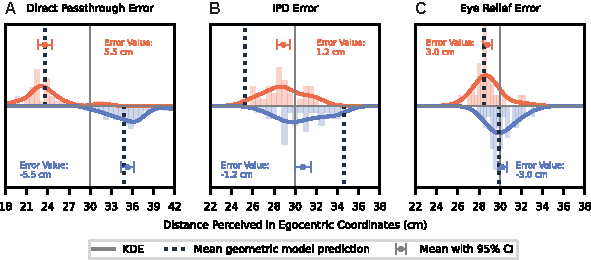
\includegraphics[width=\linewidth]{figures/reaching/egocentric_distance_summary.pdf}
	\caption{Perceived distance in egocentric coordinates induced by rendering and viewing errors compared to model predictions. Each participant's blind reaching performance is adjusted to account for their no-error blind reach baseline for \textbf{(A)} direct passthrough error, \textbf{(B)} IPD error, and \textbf{(C)} eye relief error. For each, the red histogram shows individual data (n=32) for positive error while the yellow histogram is for negative error. A kernel density estimate (KDE) is shown to visualize the distribution. \textbf{(A)} and \textbf{(B)} replot data from Figure \ref{fig:reaching_HMD_coordinates}A-B (right most data points) since HMD coordinate system overlaps with egocentric coordinate system for those two error types. Our model predictions in egocentric coordinates provide good account of the data for direct passthrough error and eye relief error, but not for IPD error. A statistically significant effect is found in all three conditions when using a general linear mixed model to examine the relationship between error magnitudes and reach accuracy.}
	\label{fig:reaching_egocentric_coordinates}
\end{figure}


\paragraph{Eye Relief Error}
Eye relief errors produced a significant linear shift in perceived distance ($\beta = -0.23, t = -5.38, p < 0.0001$). A $+3$~cm error (eyes closer to display) caused the target to appear closer than intended. Conversely, a $-3$~cm error (eyes further from display) resulted in reaches that appeared accurate in the egocentric frame (Figure~\ref{fig:reaching_egocentric_coordinates}C). 

This apparent accuracy is due to a cancellation effect at this specific target distance: the \textit{optical error} (which geometrically pushes the virtual image away) is effectively neutralized by the \textit{egocentric frame shift} (the user standing $3$~cm further back). Although these factors canceled out at $30$~cm, the linear model confirms that our geometric predictions accurately account for the underlying trend in both positive and negative directions.